\documentclass[ 12pt ]{article}
\usepackage{amsmath, amsthm, amssymb, csquotes, enumitem, graphicx, listings, mathrsfs}
\usepackage[margin=0.5in]{geometry}
\graphicspath{ ./ }

\newcounter{lecture_num}
\theoremstyle{plain}

\theoremstyle{plain}
\newtheorem{theorem}{Theorem}[lecture_num]
\newtheorem{proposition}[theorem]{Proposition}
\newtheorem{lemma}[theorem]{Lemma}
\newtheorem{corollary}[theorem]{Corollary}

\theoremstyle{definition}
\newtheorem{definition}[theorem]{Definition}
\newtheorem{notation}[theorem]{Notation}
\newtheorem*{notation*}{Notation}
\newtheorem{observation}[theorem]{Observation}
\newtheorem*{observation*}{Observation}
\newtheorem{question}[theorem]{Question}
\newtheorem*{question*}{Question}

\theoremstyle{remark}
\newtheorem{remark}[theorem]{Remark}
\newtheorem{example}[theorem]{Example}
\newtheorem*{example*}{Example}

\begin{document}

\noindent Landon Fox \\
\noindent Math 440 \\
\noindent February 15, 2021

\begin{center}
	\Large Lecture Summary Week 3
\end{center}

\setcounter{lecture_num}{7}
\setcounter{theorem}{0}
\section*{Lecture 7}

\subsection*{Topological Spaces}

\begin{theorem}
	Let $X$ be a set and $\mathcal{T} \subseteq 2^X$. Then the two following statements are equivalent.
	\begin{itemize}
		\item If $\{ U_1, \hdots, U_m \}$ is a collection of subsets of $X$ such that $U_i \in \mathcal{T}$ for all $i = 1, \hdots, m$, then $$\bigcap_{i = 1}^m U_i \in \mathcal{T}.$$
		\item For all $U, V \in \mathcal{T}$ it follows that $U \cap V \in \mathcal{T}$.
	\end{itemize}
\end{theorem}

\begin{proposition}
	Let $(X, \mathcal{T})$ be a topological space and $A \subseteq X$. Further, let $\mathcal{T}_A = \{ U \cap A : U \in \mathcal{T} \}$. Then $(A, \mathcal{T}_A)$ is a topological
	space. The topology $\mathcal{T}_A$ is called the \textbf{subspace topology} on $A$.
\end{proposition}

\begin{example*}
	\textbf{Proposition 7.2} provides some interesting examples of topological spaces.
	\begin{itemize}
		\item The plot of a function, $\mathrm{plot}( f : \mathbb{R} \to \mathbb{R} ) \subseteq \mathbb{R}^2$, a subspace of the Euclidean topology.
		\item The 2-sphere, $S = \{ (x, y, z) \in \mathbb{R}^3 : x^2 + y^2 + z^2 = 1 \} \subseteq \mathbb{R}^3$.
		\item Knots in $\mathbb{R}^3$, below are some examples.
			\begin{center}
				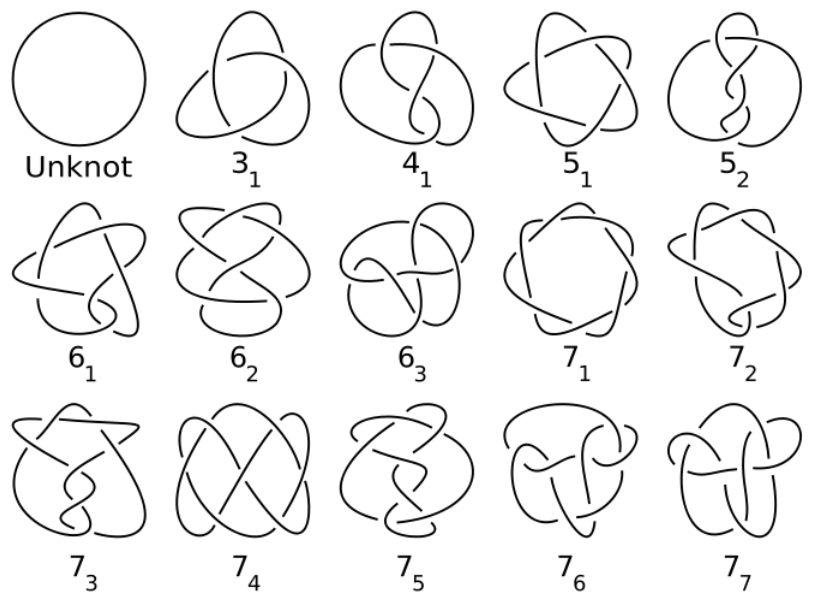
\includegraphics{Capture}
			\end{center}
	\end{itemize}
\end{example*}


\setcounter{lecture_num}{8}
\setcounter{theorem}{0}
\section*{Lecture 8}

\subsection*{Examples}

\begin{example*}
	Some exotic examples of topological spaces include the following.
	\begin{itemize}
		\item \textbf{Ex J 2.12}: The order topology.
		\item \textbf{Ex J 2.13}: The lower and upper limit topology on $\mathbb{R}$.
		\item \textbf{Ex J 2.14}: The topologist's sine curve.
		\item \textbf{Ex J 2.15}: The infinite broom.
		\item \textbf{Ex J 2.16}: Hawaiian Earrings.
	\end{itemize}
\end{example*}

\subsection*{Closed Sets and Limit Points in Topological Spaces}

\begin{theorem}
	Let $X$ be a topological space. Then
	\begin{enumerate}
		\item $X$ and $\varnothing$ are closed subsets.
		\item Finite unions of closed subsets are closed.
		\item Arbitrary intersections of closed subsets are closed.
	\end{enumerate}
\end{theorem}

\begin{definition}
	Let $X$ be a topological space and $A \subseteq X$. A point $y \in X$ is called a \textbf{limit point} of $A$ if and only if for all subsets $U \subseteq X$ containing $y$, the
	intersection $$A \cap (U \setminus \{ y \}) \neq \varnothing.$$ Define $L(A) \subseteq X$ as the set of all limit points of $A$ contained in $X$.
\end{definition}

\begin{example*}
	Some examples of limit points of sets.
	\begin{itemize}
		\item If $A = (0, 1]$, then $0, 1 \in L(A)$.
		\item If $A = \left \{ \frac{1}{n} : n \in \mathbb{N} \right \}$, then $0 \in L(A)$.
	\end{itemize}
\end{example*}

\begin{remark}
	If $X$ is a topological space and $A \subseteq B \subseteq X$, then $L(A) \subseteq L(B)$.
\end{remark}

\begin{theorem}
	Let $X$ be a topological space and let $A \subseteq X$. Then $A$ is closed if and only if $L(A) \subseteq A$.
\end{theorem}


\setcounter{lecture_num}{9}
\setcounter{theorem}{0}
\section*{Lecture 9}

\subsection*{Closed Sets and Limit Points in Topological Spaces}

\begin{remark}
	Let $X$ is a topological space. A subset $V \subseteq X$ is open if and only if for every $y \in V$, there is an open subset $U_y \subseteq X$ such that $y \in U_y \subseteq V$
	implies that $$V = \bigcup_{y \in V} U_y.$$
\end{remark}

\begin{definition}
	Let $X$ be a topological space and $A \subseteq X$. The \textbf{closure of $A$} in $X$, denoted by $\overline{A}$, is the intersection of all closed subsets of $X$ containing $A$;
	that is $$\overline{A} = \bigcap_{ A \subseteq B \subseteq X\; \mathrm{closed} } B.$$
\end{definition}

\begin{remark}
	Let $X$ be a topological space and $A \subseteq X$. Then the following holds.
	\begin{enumerate}
		\item $\overline{A}$ is closed.
		\item If $B \subseteq X$ is closed and $A \subseteq B$, then $A \subseteq \overline{A} \subseteq B$.
		\item If $A$ is closed, then $A = \overline{A}$.
	\end{enumerate}
\end{remark}

\begin{example*}
	Examples of closure.
	\begin{itemize}
		\item In the Euclidean topology $\mathbb{R}$, if $A = (0, 1)$, then $\overline{A} = [0, 1]$.
		\item In $\mathbb{R}^2$, if $B_\epsilon(\textbf{0})$, then $\overline{B}_\epsilon(\textbf{0})$ is its closure.
		\item If $X = (\mathbb{R}, \mathcal{T}_{\mathrm{disc}})$, then $A = \overline{A}$.
		\item If $X = (\mathbb{R}, \mathcal{T}_{\mathrm{triv}})$ and $A = (0, 1)$, then $\overline{A} = \mathbb{R}$.
	\end{itemize}
\end{example*}

\begin{theorem}
	Let $A \subseteq X$ be a subset of a topological space $X$. Then $\overline{A} = A \cup L(A)$.
\end{theorem}

\end{document}
